%\documentclass[11pt]{article}
%\usepackage{graphicx}
%\usepackage{amssymb}
%\usepackage{epstopdf}
%\usepackage{doublespace}
%\DeclareGraphicsRule{.tif}{png}{.png}{`convert #1 `dirname #1`/`basename #1 .tif`.png}

%\textwidth = 6.5 in
%\textheight = 9 in
%\oddsidemargin = 0.0 in
%\evensidemargin = 0.0 in
%\topmargin = 0.0 in
%\headheight = 0.0 in
%\headsep = 0.0 in
%\parskip = 0.2in
%\parindent = 0.0in

%\newtheorem{theorem}{Theorem}
%\newtheorem{corollary}[theorem]{Corollary}
%\newtheorem{definition}{Definition}

%\title{Matrix Multiply Results}
%\author{Daniel D. Beatty}
%\begin{document}
%\maketitle

%\chapter


Each empirical result is from % either 
a series of matrix multiplications on 9 different images.  These matrices were submitted preconditioning with the wavelet transform in the 3 basic method of decomposition, wavelet pyramid, wavelet packet (full decomposition) and the $\psi^n$ decomposition.%   with wavelet packets or wavelet pyramids type wavelet transforms.  
In the end, wavelet pyramids performed poorly for any set of resolutions deeper than one in matrix multiplication.  Thus wavelet packets should not be used as a pre-conditioner to matrix multiplication.  The wavelet transform  by wavelet packets performs modestly in matrix multiplication tests, but to be effective must be reordered into $\psi^n$ structure. %require reordering to match the recursive MRE wavelet transform packet form.    
Lastly, the $psi^n$ form performs well on matrix multiply.   

The matrix multiply used in each of these cases is %a special case of matrix multiply is conducted, 
$A^2= A\cdot A$, where $A$ is $M\times N$ The general equation for evaluating the wavelet transform pyramid method is the fidelity measurement:

\[\sqrt{E(\psi_{Pr}^{-x} ( (\psi_{Pr}^x (A))^2) - A^2)} \]

Relative Fidelity measurements provide a relative standard and is more useful for general observations.  To obtain this measurement, the results are compared to standard.% reference of a standard.  
In this case, $A^2$ is the standard, and the energy difference is relative to that standard.  

\[ \sqrt {\frac{E(\psi_{Pr}^{-x} ( (\psi_{Pr}^x (A))^2) - A^2)} {E(A^2)} }  \]

%\section {Matrix Multiplication Results}
%\{tiny}

\section {Empirical Analysis: Wavelet Transform Pyramids}

Several standard images were used for measuring effect matrix multiply in each of these multiplications.  Amongst them were the artificial images such as the waterfall and the clock.  Others were actual images such as an arial view of the Pentagon, an in flight photo of an F-16, a fishing boat, an opera house, a river, and a set of bell peppers.

In first round analysis, matrix multiply was measured against the wavelet pyramids.  These showed some undesirable results.  As the decomposition proceeded deeper, the fidelity quick became unstable, and made the method unusable for matrix multiplication.  

These tables are shown below.

Sample Two: Peppers $512 \times 512$ by wavelet transform pyramid 

\begin{tabular}{llll}
{Resolution} & { Original Energy } & { 
Estimate Energy }& { 
Fidelity } \\ 
1&  12972.4& 12972.4 &  $1.26464 \cdot 10^{-13} $ \\ 
2&12972.4  & 12960.3 &  3.11211  \\ 
3& 12972.4 &12947.8  &  5.44678  \\ 
4&12972.4&12939.7&   8.43738 \\
5 &12972.4  & 12926 & 13.1662 \\
6& 12972.4& 12904.3& 19.9257 \\
7& 12972.4 & 12877.9 & 25.4429 \\
\end{tabular}


%Sample Three: Molly Holly $256 \times 256$ by wavelet transform pyramid 

%\begin{tabular}{lllll}
%{\tiny Number of Resolution} & {\tiny Original Energy }$E(O)$ & {\tiny 
%Estimate Energy }$E(\widetilde{O})$ & $(E(O)-E(\widetilde{O}))$ & {\tiny 
%Fidelity }$\sqrt{E((O)-(\widetilde{O}))}$ \\ 
%$1$ & $582.864 $ & $582.864$ &  $-9.75244\cdot 10^{-16}$ & $2.0396 \cdot 10^{-14}$ \\ 
%$2$ & $582.864 $& $583.05 $  & $-0.000319839$ & $1.19806 $  \\ 
%$3$ &  $582.864$ & $582.613$ & $0.000430391$  & $2.18712$ \\ 
%$4$ & $582.864$ & $579.473$ & $0.00581664$ &  $3.19317$ \\ 
%$5$ & $582.864$ & $576.72$ & $0.0105413$ & $4.82652$ 

%\end{tabular}


Sample Four: Waterfall $512 \times 512$ by wavelet transform pyramid 

\begin{tabular}{llll}
{ Resolution} & { Original Energy }& { 
Estimate Energy } &  { 
Fidelity } \\ 
$1$&  $6630.76$ & $6630.76$&  $9.37836e-14$ \\ 
$2$& $6630.76$ & $6629.92$  &  $1.20049$ \\ 
$3$& $6630.76$ & $6626.6$   & $2.37529$ \\ 
$4$& $6630.76$ & $6619.14$  & $3.9194$ \\ 
$5$& $6630.76$ & $6595.14$  &  $6.63615$\\ 
$6$& $6630.76$ & $6579.62$  & $9.48774$ \\ 
$7$& $6630.76$ & $6567.17$  &  $12.1211$
\end{tabular}

\section {Empirical Analysis: Wavelet Transform Packets}
The primary example shown is from the Peppers image.  Although, all nine of the images used for this thesis could have been used, all of them exhibit similar qualities.   After, two resolutions the 2-D MRE becomes unstable for matrix multiplication.  It misplaces sections to where random noise in those sections would be just useful as the actual information contained in those sections.  
%These examples were chosen arbitrarily from a selection images with fidelity-issued features.  In other-words, a loss in fidelity is noticed by the human eye.  Also, size was considered in these measurements as well.  

Sample One: Peppers $512 \times 512$ by wavelet transform packet 

\begin{tabular}{llll}
{ Resolution } &  {Original Energy }  &{ Estimate Energy }  & {Fidelity} \\ 
$1$ & $12972.4$ &  $12972.4$ &  $1.26464e \cdot 10^{-13}$\\ 
$2$ & $12972.4$ & $12972.4$ &  $0.059622$ \\ 
$3$ & $12972.4$ & $12972.4$ &  $0.072957$  \\ 
$4$& $12972.4$  & $12972.4$  & $0.0849579$  \\ 

$5$& $12972.4$  & $12972.4$  & 0.09721  \\ 

$6$& $12972.4$  & $12972.4$ &  $0.104528$  \\ 

$7$& $12972.4$  & $12972.4$ &  $0.119789$  \\ 

\end{tabular}

\section {Empirical Results on the Psi-N Wavelet Transform Method}
The Psi-N transform clearly produces better results as shown in all examples of the wavelet transform.  Trade off issues start to appear when comparing the number of resolution levels to apply as opposed to a spare filter threshold.   

In these next examples, resolution levels 1 through 7 are examined by removing data based on energy level.  The method used is to strictly remove the lower threshold of energy from the matrix at large.  %The second method removes energy first by eliminating whole segments.  The third is a hybrid, removing first the segments at large and then filtering on the threshold segment.  
The range of energy thresholds vary from 0 to $\frac{9}{10}$. 

The reasoning for any of these schemes is to establish sparse representations of the matrix.  In these sparse representation, only the above threshold elements are used.   These representations are useful for sparse matrix multiplication since only the above threshold elements need be multiplied thus reducing the number of multiplications (operations at large) performed.  

%\subsubsection {Strict Lower Threshold Scheme: The Darwin Filter}
This filter is appropriately named for allowing the strongest elements to survive and weaker ones to be reduced to zero.  This particular Darwin Filter is applied through out the matrix.  In order to find the element that is the threshold element, each element in the matrix is squared, placed in a one dimensional array, and then sorted in the array from least to greatest.  %Lastly the summing loop is applied to the array, and is stopped when either entire array is processed or the sum has reached the threshold value.  The threshold value is established by the energy of the matrix multiplied by the energy percentage to be removed.  
Lastly, two method exist to find the threshold value in the array of values.  One is to sum up values until the threshold energy level has been reached.  Another is to take element relative to the percentage threshold desired.  The relative percentage method is simpler, by performing one division on the energy array size and a look up for the value in the energy array.  

Once found, the filter threshold is used to filter out elements whose squared value is less than the threshold.  Those elements that are less are made to be zero.   Those that are above the threshold are left alone.  

For this experiment both matrix operands have the filter applied.  It should be noted that for the BLAS level three matrix multiply, this filtering scheme need only be applied to the first matrix operand.   Applying this filter to the second is simply unnecessary since the method states that the second matrix can be dense.  

The pattern of fidelity loss has a dramatic climb in the first $\frac{1}{20}$ of energy loss.  From $\frac{1}{20}$ th to $\frac{1}{2}$ the fidelity stays roughly within the same order of magnitude.  After this there is a sharp rise until all fidelity is lost.  

\begin{figure}
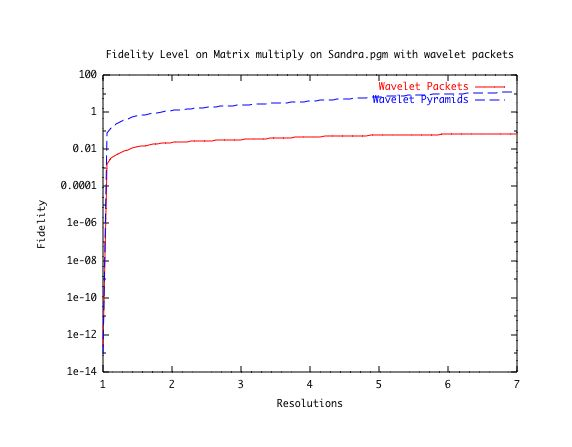
\includegraphics [width=7in]{sandrapyrpackresults.jpg}
\caption{This fidelity level graph shows that the wavelet transform packet method as a preconditioner to matrix multiply is not reliable past the first resolution. The wavelet packet produces marginal results mostly due sections being placed out of order.}
\label{packetresultsstraight}
\end{figure}






\begin{figure}
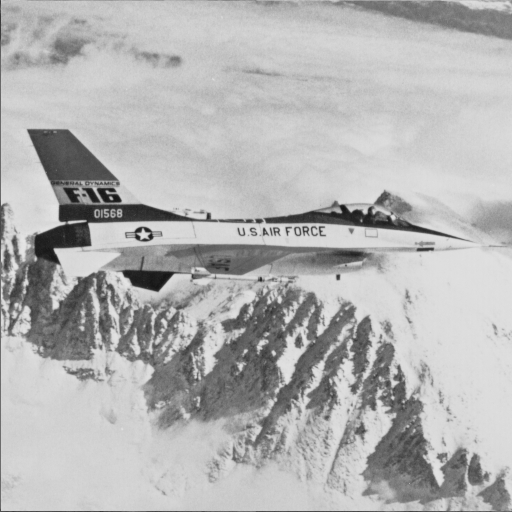
\includegraphics [width=3in]{f16.jpg}
\caption{This image is a photo of an F-16 fighter jet provided Courtesy of the Signal and Image Processing Institute at the University of Southern California.  \cite{f16}}
\label{image f16}
\end{figure}


\begin{figure}
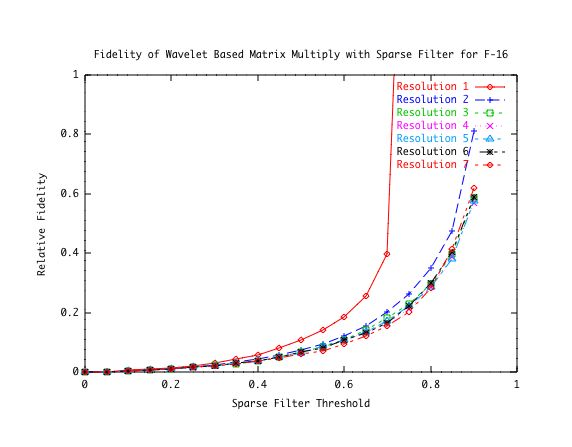
\includegraphics [width=5.5in]{f16resultsA.jpg}
\caption{This fidelity level graph shows that Psi Wavelet Transform (full decomposition) approximation error in matrix multiplication.  This graph in particular was obtained by multiplying the F-16 image by itself with various resolution levels of Wavelet Transforms applied. \cite{f16} }
\label{image f16 fidelity}

\end{figure}

\begin{figure}
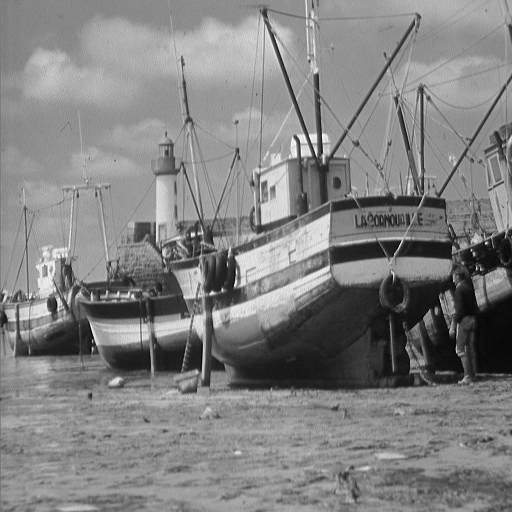
\includegraphics [width=3in]{fishingboat.jpg}
\caption{This image is a photo of an F-16 fighter jet provided Courtesy of the Signal and Image Processing Institute at the University of Southern California.  \cite{fishingboat}}
\label{image_fishingboat}
\end{figure}



\begin{figure}
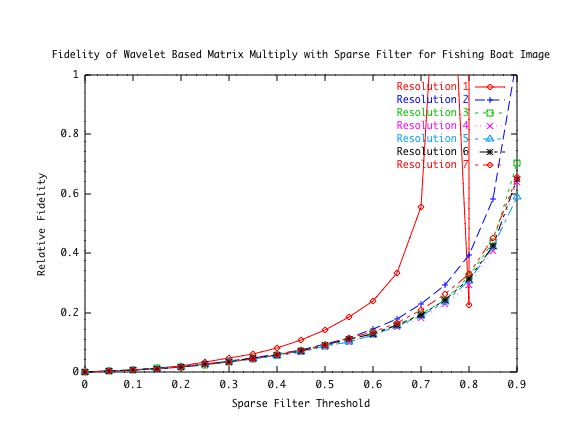
\includegraphics [width=5.5in]{fishingboatresultA.jpg}
\caption{This fidelity level graph shows that Psi Wavelet Transform (full decomposition) approximation error in matrix multiplication.  This graph in particular was obtained by multiplying the Fishing Boat image by itself with various resolution levels of Wavelet Transforms applied. \cite{fishingboat}  }
\label{image_fishingboat_fidelity}
\end{figure}


\begin{figure}
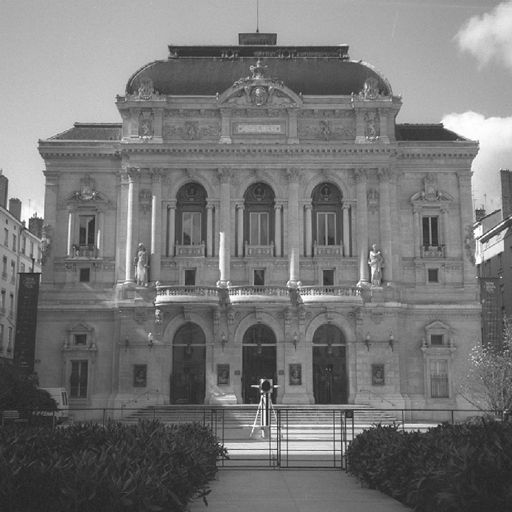
\includegraphics [width=3in] {opera.jpg}
\caption {This image is a photo of the Opera House in Lyon \cite{opera}}
\label{Opera House}
\end{figure}

\begin{figure}
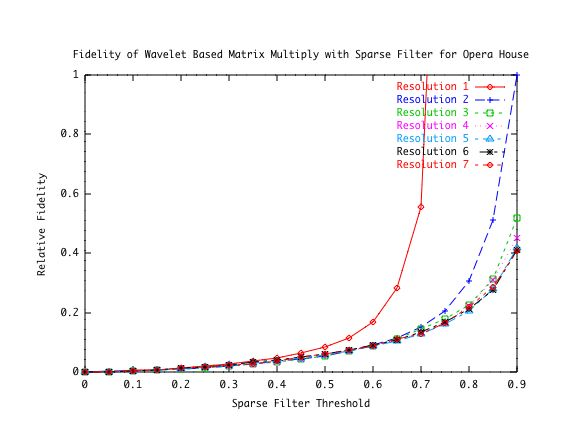
\includegraphics [width=5.5in]{operaresultsA.jpg}
\caption{This fidelity level graph shows that Psi Wavelet Transform (full decomposition) approximation error in matrix multiplication.  This graph in particular was obtained by multiplying the Opera House image by itself with various resolution levels of Wavelet Transforms applied.  }
\label{image_opera_fidelity}
\end{figure}

\begin{figure}
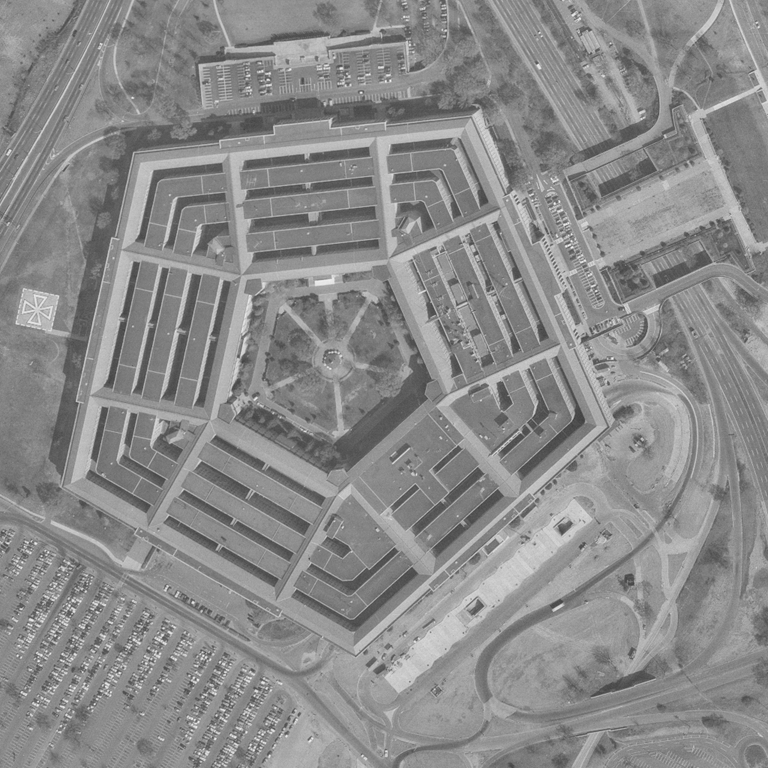
\includegraphics [width=3in]{pentagon.jpg}
\caption{This image is an ariel photo of an Pentagon provided Courtesy of the Signal and Image Processing Institute at the University of Southern California.  \cite{pentagon}}
\label{image fishingboat}
\end{figure}

\begin{figure}
\includegraphics [width=5.5in]{pentagonresultsA.jpg}
\caption{This fidelity level graph shows that Psi Wavelet Transform (full decomposition) approximation error in matrix multiplication.  This graph in particular was obtained by multiplying the Pentagon image by itself with various resolution levels of Wavelet Transforms applied. \cite{Pentagon} }
\label{image_pentagon_fidelity}
\end{figure}

\begin{figure}
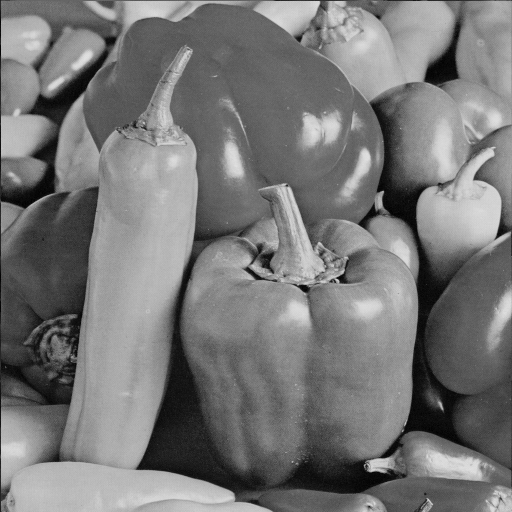
\includegraphics [width=3in]{peppers.jpg}
\caption{This image is an ariel photo of  ``Peppers'' provided Courtesy of the Signal and Image Processing Institute at the University of Southern California.  \cite{peppers}}
\label{image Peppers}
\end{figure}

\begin{figure}
\includegraphics [width=5.5in]{peppersresultsA.jpg}
\caption{This fidelity level graph shows that Psi Wavelet Transform (full decomposition) approximation error in matrix multiplication.  This graph in particular was obtained by multiplying the Peppers image by itself with various resolution levels of Wavelet Transforms applied. \cite{peppers} }
\label{image_peppers_fidelity}
\end{figure}

\begin{figure}
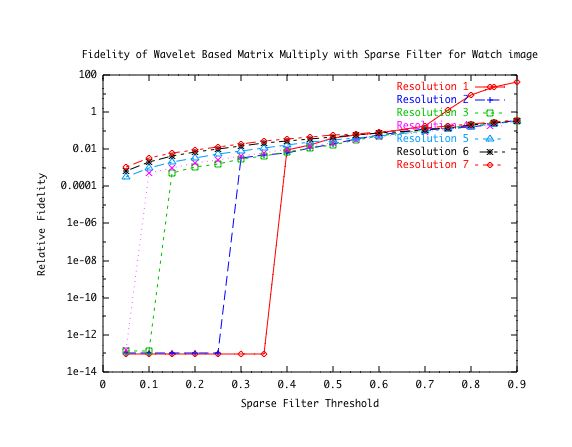
\includegraphics [width=6in]{watchResultsA.jpg}
\caption{This fidelity level graph shows that Psi Wavelet Transform (full decomposition) approximation error in matrix multiplication.  This graph in particular was obtained by multiplying the Watch image by itself with various resolution levels of Wavelet Transforms applied.  \cite{watch} }
\label{image_watch_fidelity}
\end{figure}

\begin{figure}
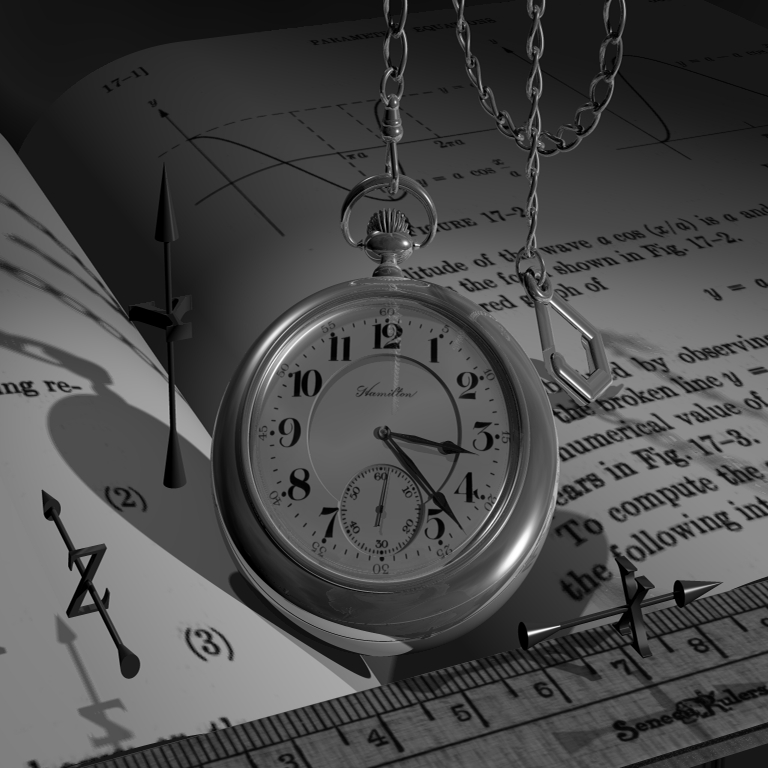
\includegraphics [width=3in]{watch.jpg}
\caption{``Pocket Watch on a Gold Chain. Copyright image courtesy of Kevin Odhner''   \cite{watch}}
\label{image Peppers}
\end{figure}

\begin{figure}
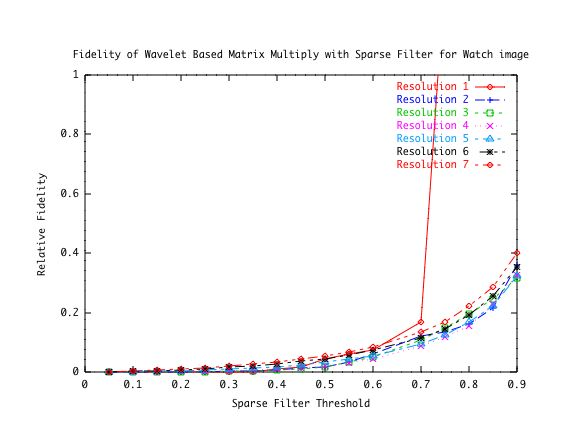
\includegraphics [width=4in]{watchResultsB.jpg}
\caption{This fidelity level graph shows that Psi Wavelet Transform (full decomposition) approximation error in matrix multiplication.  This graph in particular was obtained by multiplying the Watch image by itself with various resolution levels of Wavelet Transforms applied.  \cite{watch}  }
\label{image_watch_fidelity}
\end{figure}

\begin{figure}
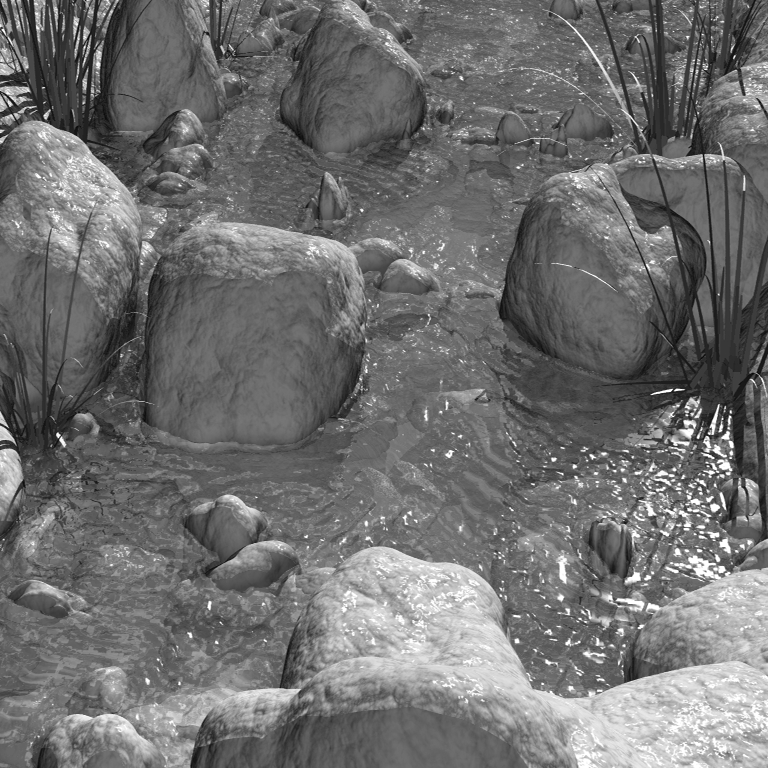
\includegraphics [width=3in]{water.jpg}
\caption{This image is an ariel photo of  ``Always running, never the same....'' provided Courtesy of the Jaime Vives Piqueres.  \cite{water}}
\label{image Peppers}
\end{figure}

\begin{figure}
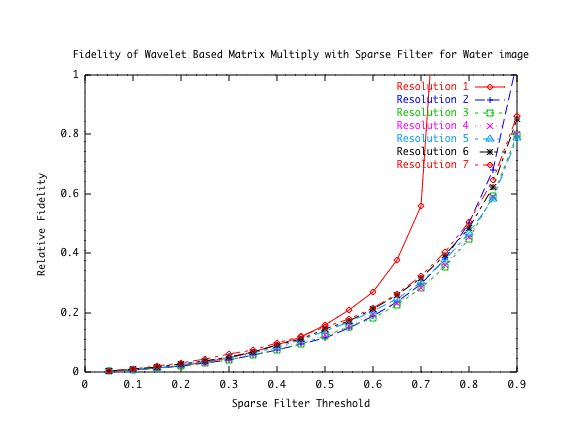
\includegraphics [width=6in]{waterResultsA.jpg}

\caption{This fidelity level graph shows that Psi Wavelet Transform (full decomposition) approximation error in matrix multiplication.  This graph in particular was obtained by multiplying the Water image by itself with various resolution levels of Wavelet Transforms applied.  \cite{watch} }
\label{image_waterfall_fidelity}
\end{figure}


\begin{figure}
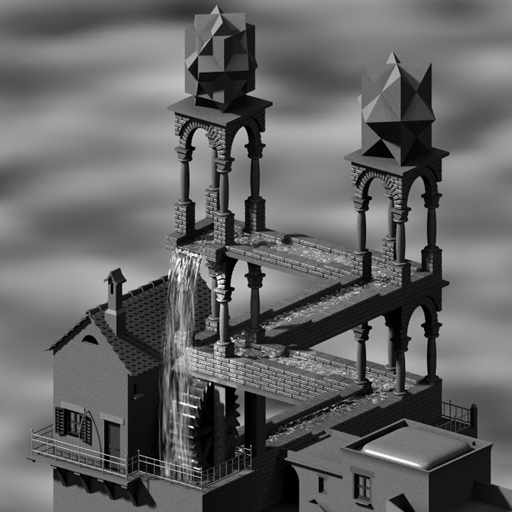
\includegraphics [width=3in]{waterfall.jpg}
\caption{"This is a raytraced version of M.C.Escher's (1898-1972) famous lithography
'Waterfall' (1961), which again is based on a spatial illusion drawen by the
mathematician Roger Penrose." \cite{waterfall} }
\label{image waterfall}
\end{figure}
\begin{figure}
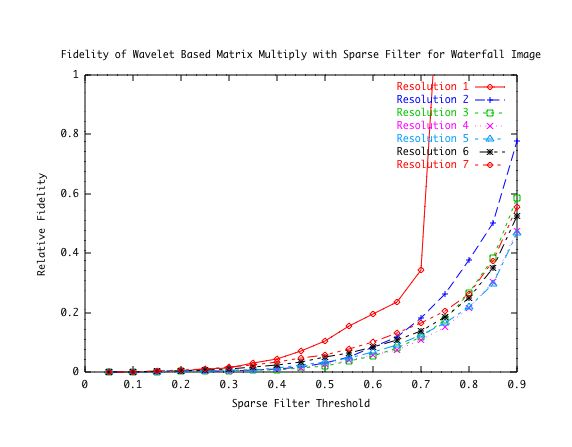
\includegraphics [width=3in]{waterfallResultsA.jpg}
\caption{This fidelity level graph shows that Psi Wavelet Transform (full decomposition) approximation error in matrix multiplication.  This graph in particular was obtained by multiplying the Waterfall image by itself with various resolution levels of Wavelet Transforms applied.  \cite{waterfall} }
\label{image_waterfall_fidelity}
\end{figure}

%\begin{thebibliography}{99}
%\bibitem {waterfall} Sascha Ledinsky \textsl{Waterfall} http://oz.irtc.org/ftp/pub/stills/1998-10-31/waterfa1.txt Internet Raytracing Competition copyright October 31, 1998
%\bibitem {water} Jaime Vives Piqueres \textsl {Always running, never the same...} http://oz.irtc.org/ftp/pub/stills/1998-10-31/running.txt  Internet Raytracing Competition copyright October 31, 1998
%\bibitem {watch} Kevin Odhner \textsl {Pocket Watch on a Gold Chain} 
%\bibitem {opera} fabien a. p. petitcolas {Opera House of Lyon} open domain
%\bibitem {pentagon} Signal and Image Processing Institute at the University of Southern California \textsl{Pentagon} The copyright status of this images in unclear.
%\bibitem {f16}  Signal and Image Processing Institute at the University of Southern California \textsl{F-16}
% The copyright status of this images in unclear.
%\bibitem  {peppers} Signal and Image Processing Institute at the University of Southern California \textsl {Peppers} The copyright status of this images in unclear.
%\bibitem {fishingboat} Signal and Image Processing Institute at the University of Southern California \textsl {Fishing Boat} The copyright status of this images in unclear.

%\end {thebibliography}
% \end{document} 